
%  LP: la partie commentee ci-dessous a ete copié dans le fichier
%  ``reference_flux.tex'' (peut etre supprimee ici)

%\subsubsection{Reference flux densities of secondary calibrators}
%\label{se:fluxSec}
%(revised by JFL Aug 2017 - must remove the old version in photometry-HA.tex)
%

%++ SPIRE refer.

%The secondary calibrator MWC349A is a young Be star, part of a stellar binary system, surrounded by a disk. Its radio
%continuum emission originates in an ionized bipolar outflow (Tafoya et al 2004).
%MWC349 has been monitored with the  Plateau de Bure interferometer and VLA,
%and shown to be stable in time and only slightly angularly resolved, making it a point source
%for the 30-metre telescope. We have computed its flux densities at the NIKA2 reference frequencies 150 and 260 GHz with 
%$S_\nu = 1.16\pm0.01 \times (\nu/100 \rm{GHz})^{0.60\pm0.01}$ provided by this monitoring
%\footnote{http://www.iram.fr/IRAMFR/IS/IS2012/presentations/krips-fluxcalibration.pdf} and
% private communication by Krips (2017) (see SED in her Fig.~\ref{fig:Krips2017}).
%
%The secondary calibrator CRL2688 is an Asympotic Giant Branch star. Its radio continuum emission is mostly
%from circumstellar dust and is somewhat extended  (Knapp et al 1994).
%Its flux densities at $850\mu$m  and $450\mu$m  have been stable at the 5\% level as monitored by SCUBA2 in 2011-2012
%(Dempsey et al 2013). We have extrapolated their flux densities to  150 and 260 GHz
%with the power law $S_{\nu} \propto \nu^{\alpha}$ and index $\alpha=2.44\pm0.18$ derived from their SCUBA2 measurements.
%
%\begin{table}[h]
%%\centering
%\caption[]{Reference flux densities of secondary calibrators at the NIKA2 reference frequencies 150 and 260 GHz.}
%\begin{tabular}{|l|c|c|c|l|}
%\hline
%\multicolumn{1}{|c}{}  & \multicolumn{3}{|c}{flux  densities (Jy)} & \multicolumn{1}{|c|}{}  \\
%\hline
%         &    A1 \& A3       &  A2             &          &   Ref. \\
%         &  260GHz           &  150GHz         & $\alpha^1$ &      \\
%\hline
%MWC349   &   $2.06\pm0.04$  &  $1.48\pm0.02$ &  $+0.60\pm0.01$      &  PdB (priv. com., Krips 2017)    \\
%NGC7027  &   $3.46\pm0.11$   &  $4.26\pm0.24$  &  $-0.34\pm0.10$     &  Hoare et al 1992       \\
%CRL2688  &   $2.91\pm0.23$   &  $0.76\pm0.14$  &  $+2.44\pm0.18$     &  Dempsey et al 2013  \\
%\hline
%\end{tabular}
%{\scriptsize $^1$ Spectral index is defined as $S_{\nu} \propto \nu^{\alpha}$. Uncertainties of flux densities extrapolated
%at 150 and 260 GHz include contribution of the uncertainty on $\alpha$.}
%\label{tab:flux_ref_sec}
%\end{table}
%% cahier I p. 128 et 129.
%
%The secondary calibrator NGC7027 is a young, dusty, carbon rich Planetary Nebula with an ionized core.
%It is extended in the continuum and molecular lines (Bieging et al 1991), and  is not a point source
%for the 30-metre telescope.
%Its  most recent flux densities are reported at $1100\mu$m  and $2000\mu$m by Hoare et al (1992). It has been reported
%to decrease by $\sim$ 0.145 percent/yr in the optically thin part of its spectrum above  $6$ GHz from VLA
%observations (Zijlstra, van Hoof \& Perley 2008, and Hafez et al, 2008) that makes these flux densities uncertain
%by 3.6\% currently. Its SED from cm wavelengths to optical is also presented in Hafez, Y.A. et al (2008).
%Its flux densities have been extrapolated to 150 and 260 GHz and the modelled decrease since 1992 included.
%
%All these extrapolated flux densities are in Table~\ref{tab:flux_ref_sec}.
%
%\begin{figure}[h]
%\begin{center}
%  \includegraphics[clip, angle=0, scale=0.4]{Figures/MWC_349_pap-flux.eps}
%  \caption{SED of MWC349 from its flux density monitoring at PdB and VLA by Krips (2017) (private commubication).
%  Symbols are for primary calibrators used (Uranus, Neptune and Mars).}
%\label{fig:Krips2017}
%\end{center}
%\end{figure}
%

\subsection{Aperture photometry}
\label{S:ApPh}

Photometry is most advantageously done by PSF fitting in the map when the observed source is a point-source and the PSF profile 
well known. When any of these conditions are not met, aperture photometry is the most cautious way to proceed.
The 30-metre PSF depends on the alignment between the telescope optical axis and the instrument 
after its last installation in January 2017, and is not well known. Hence, we have used aperture photometry to
caracterize the stability of the Jy scale in monitoring the
primary and secondary calibrators observed during the commissioning runs 9 and 10.
We describe first how we have implemented aperture photometry.

First, all observations (beammaps and $8' \times 5'$ otf's) were processed 
with the pipeline set up with the parameters of Table~\ref{tab:Pipe} to produce the intensity map of each array.
We stress that the  gain-elevation curved of EMIR implemented in the pipeline has NOT been turned on for our processing.

\begin{table}[h]
\centering
\caption[]{Pipeline set-up.}
\begin{tabular}{|l|c|c|}
\hline
                      &    run 9                             &  run  10                   \\
\hline
kidpar                &  {\scriptsize kidpar-best3files-FXDC0C1-GaussPhot} &  {\scriptsize kidpar-n2r10-calib.fits}   \\
Decorrelation method  &  {\scriptsize COMMON-MODE-ONE-BLOCK} &    {\scriptsize COMMON-MODE-ONE-BLOCK}    \\
Opacity               &  {\scriptsize  l.o.s}                &  {\scriptsize l.o.s}     \\
Sky Projection        &  {\scriptsize RADEC}                  &  {\scriptsize RADEC}     \\
a priori mask         &  {\scriptsize   $50''$}              &  {\scriptsize $100''$}  \\
Iteration in mapping  &  {\scriptsize  None}                 &  {\scriptsize None}     \\
Elevation gain curve  &  {\scriptsize  None}                 &  {\scriptsize None}      \\
\hline
\end{tabular}
\label{tab:Pipe}
\end{table}

The total flux density of a source  measured over an aperture  is :

\begin{equation}
S_{\nu} = \sum_{m} \sum_{n}  I_{m,n} ({\rm Jy/beam}) \times {dx^2 \over {\Omega_{true}(\nu, r_{max})}}
\label{eq:ApPh}
\end{equation}

\noindent  $I_{m,n}$ is the brightness in Jy/beam in each pixel of the NIKA2 map, indices
$m,n$ are such that $dx \times \sqrt{(m-m_c)^2 + (n-n_c)^2} < 150''$ (aperture radius), $dx$ is the pixel size,
$m_c,n_c$ are at the map center, $\Omega_{true}(\nu, r_{max})$ is the solid angle of the total beam and named $true$ by usage.
Prior to summation of all intensities within the aperture, each $I_{m,n}$ 
must be converted from its natural unit Jy/beam to Jy/pixel. We stress that beam in unit Jy/beam
stands for the total beam including main beam and side lobes (sometimes called error beam).

The solid angle of the total beam is defined by :

\begin{equation}
 \Omega_{true} (\nu,r_{max}) = \int_0^{2\pi} \int_0^{r_{max}} B(\nu, r) 2 \pi r dr
\label{eq:Otrue}
\end{equation}

\noindent where $B(\nu,r)$ is the radial profile of the source obtained in azimuthally averaging brigthness over narrow annuli
$dr$ in width, and normalised so that B(0)=1 (R. Adam's thesis (2016) or J.D. Kraus (1980)).
This assumes that the PSF is azimuthally symmetric. 
We have used $r_{max}=250''$ which is the maximum extent allowed by the size of the maps acquired during observations.
We have estimated that only ????? \%  of the incident power resides in side lobes beyond $r_{max}$ is missed,
see Greve et al (1998) and Kramer et al (2013).

The excess of the total beam relative to the Gaussian beam is the ratio
$\Omega_{true} / 2 \pi (\sigma_{Gauss})^2$, with  $\sigma_{Gauss}$ derived from $FWHM$ which can be determined
from the NIKA2 map if the source is point-like.


\subsection{Solid angle of the total beam}
\label{S:solang}

Uranus and Neptune are the best sources to caracterize the intrument because
they are significantly stronger than the other calibrators.                                                               
The solid angle $\Omega_{true}$ of the total beam has been computed with  eq.~\ref{eq:Otrue}
and its excess relative to the Gaussian beam derived
for each  observation of Uranus or Neptune in  runs 9 and 10 under  a broad range of atmospheric conditions
($0.05 < \tau_{1mm} < 0.65$)  and their histogram are shown in Fig. ~\ref{fig:Otrue}.

\begin{figure}[h]
\begin{center}
  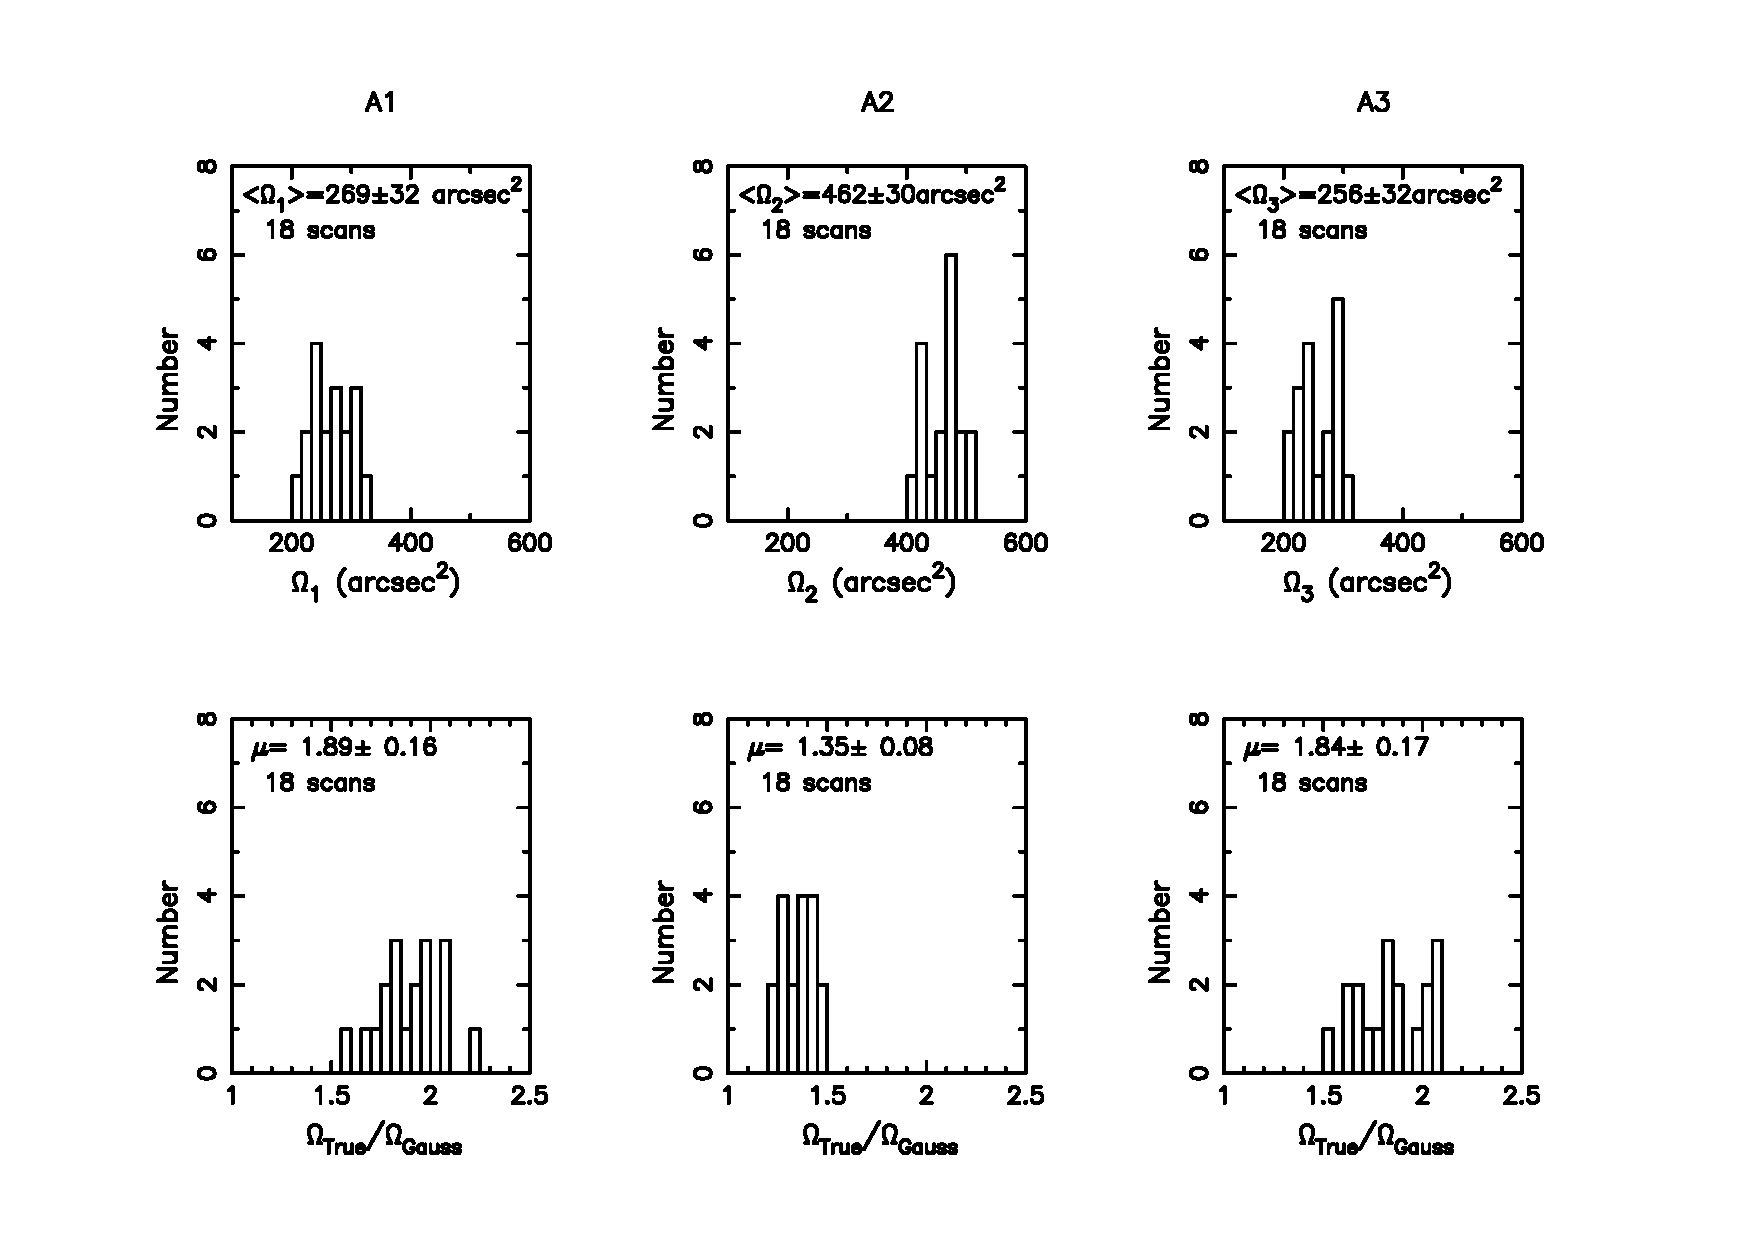
\includegraphics[clip, angle=0, scale=0.6]{Figures/Hist_omega_true_and_excess.pdf}
  \caption{Solid angle of the total beam ($\Omega_{true}$) and its excess relative to the Gaussian beam
   ($\Omega_{true} / 2 \pi (\sigma_{Gauss})^2$ for the 18 observations of Uranus and Neptune during runs 9 and 10.
   Histogramms, mean and rms for each array.}
\label{fig:Otrue}
\end{center}
\end{figure}

We have found that the solid angle of the total beam is slightly variable and its mean and rms are
$269\pm32$, $462\pm30$, and $256\pm32$ arcsec$^2$ for arrays 1, 2, and 3, respectively, and, hence,
that $\Omega_{true}$ is proportional to $\nu^{-1}$ as expected. Also, the excess of the total beam
relative to the Gaussian beam (ratio of solid angles) has means and rms
of $1.89\pm0.16$, $1.35\pm0.08$ and $1.84\pm0.17$, for arrays 1, 2 and 3, respectively.
We note these ratios provide
the beam efficiencies (ratio of powers between main beam  and total beam). They
are $\sim 55$ \% at 1mm ($1/1.87 \times 100$) and $\sim 70$ \% at 2mm ($1/1.35 \times 100$)
over the same extent $r_{max}=250''$ and are consistent with their direct determination in \S~\ref{se:beams}.
 We provide the  distributions of $\Omega_{true}$ and excesses for
 the 18 observations of Uranus and Neptune during runs 9 and 10 in Figure ~\ref{fig:Otrue}. 

We have searched for any systematics in these estimations of $\Omega_{true}$ with respect to elevation,
opacity,  and transmission ($exp(-\tau/sin(elev)$) in Fig.~\ref{fig:Osystematics}.
Over the limited range of elevations between  33$^{\circ}$ and 58$^{\circ}$ covered by the 18 observations,
there is no definitive correlation although
a 15\% increase of $\Omega_{true}$ at small opacity ($<0.15$) and, consequently,
at high transmission ($> 0.8$), is hinted by inspection of the plots.
This effect is not understood and under investigation. 

\begin{figure}[h]
\begin{center}
  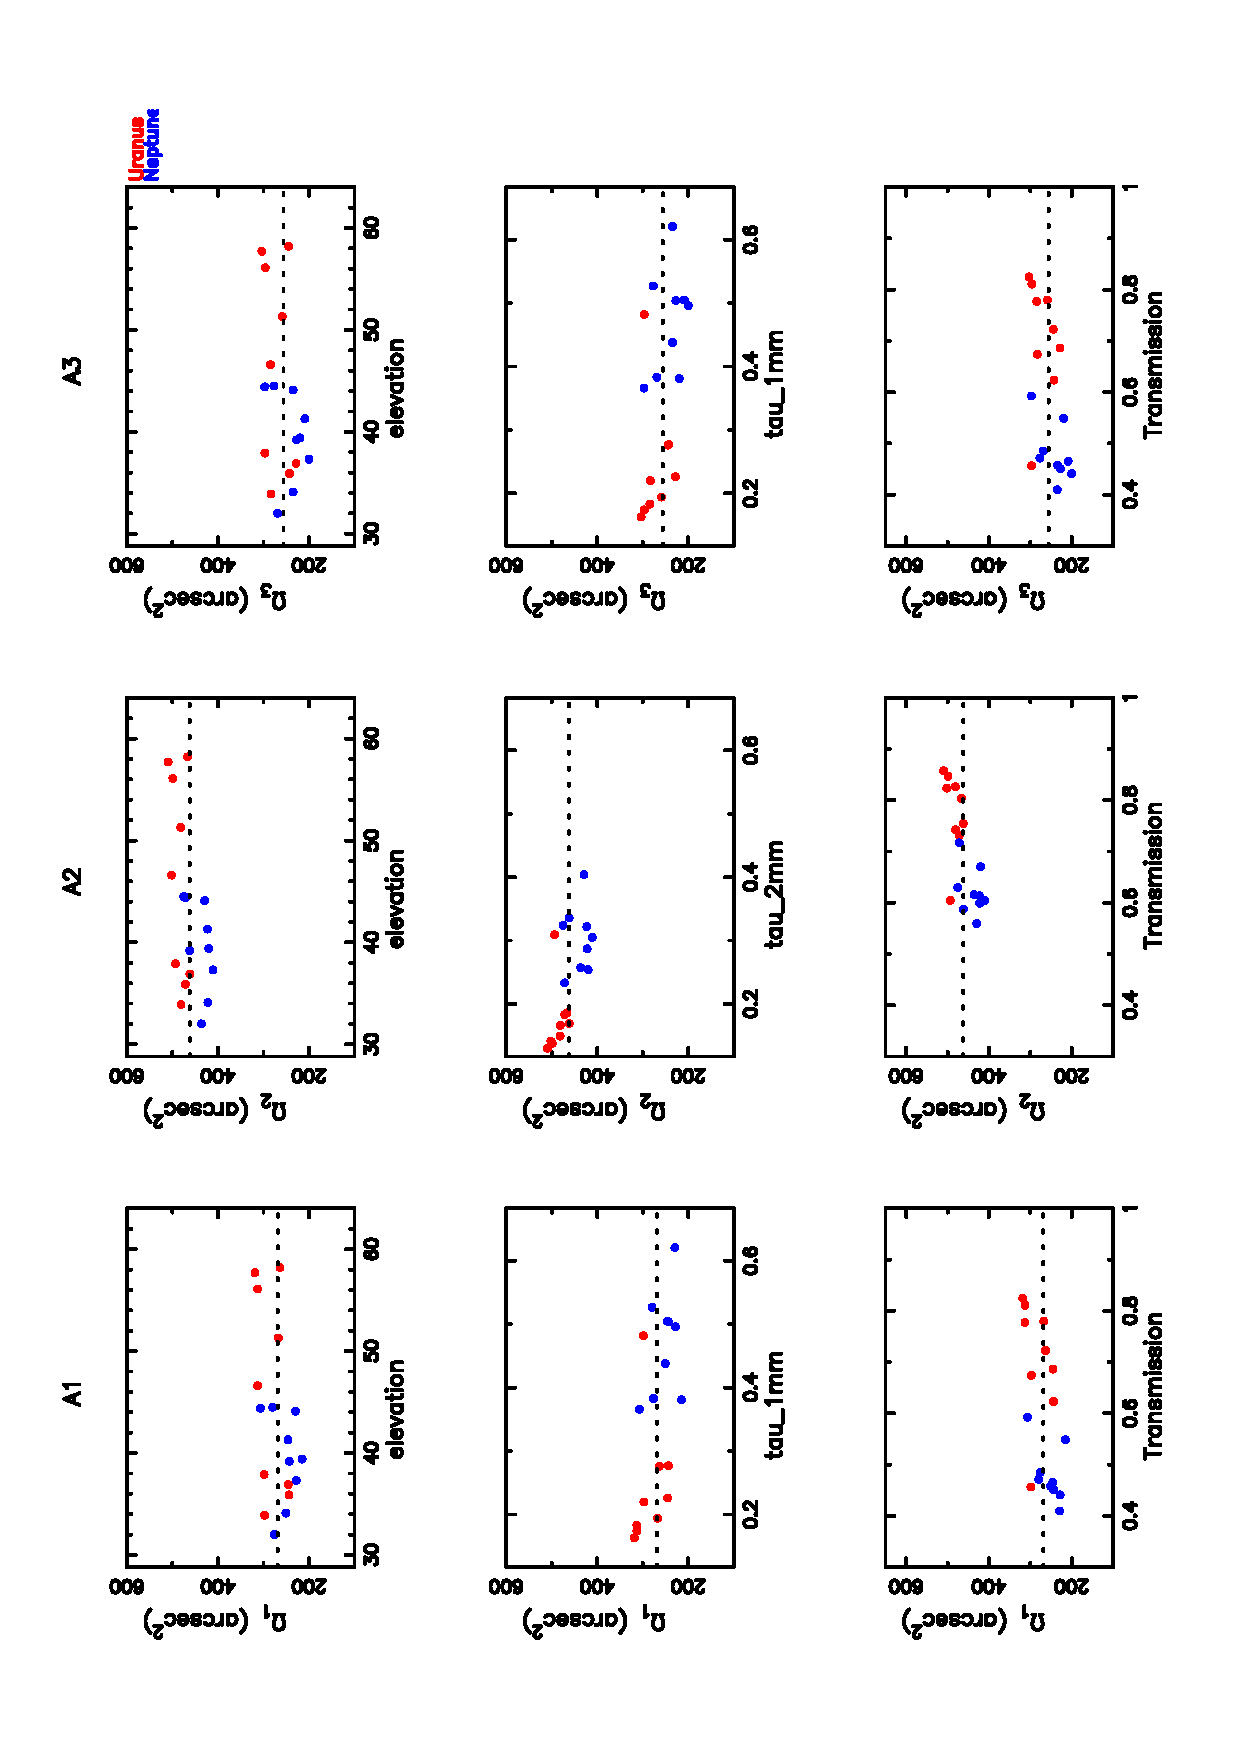
\includegraphics[clip, angle=-90, scale=0.6]{Figures/Omega_True_vs_elev_tau_transmission.pdf}
  \caption{Search for systematics in the solid angle of the total beam $\Omega_{true}$
   with respect to elevation, opacity and transmission ($exp(-\tau/sin({\rm elev})$) of the 18 observations
   of Uranus and Neptune during runs 9 and 10. There is no definitive correlation although a 15\% increase
   of $\Omega_{true}$ at small opacity ($<~0.15$), and consequently
  at high transmission ($>~0.8$), is hinted.}
\label{fig:Osystematics}
\end{center}
\end{figure}


\begin{figure}[h]
\begin{center}
  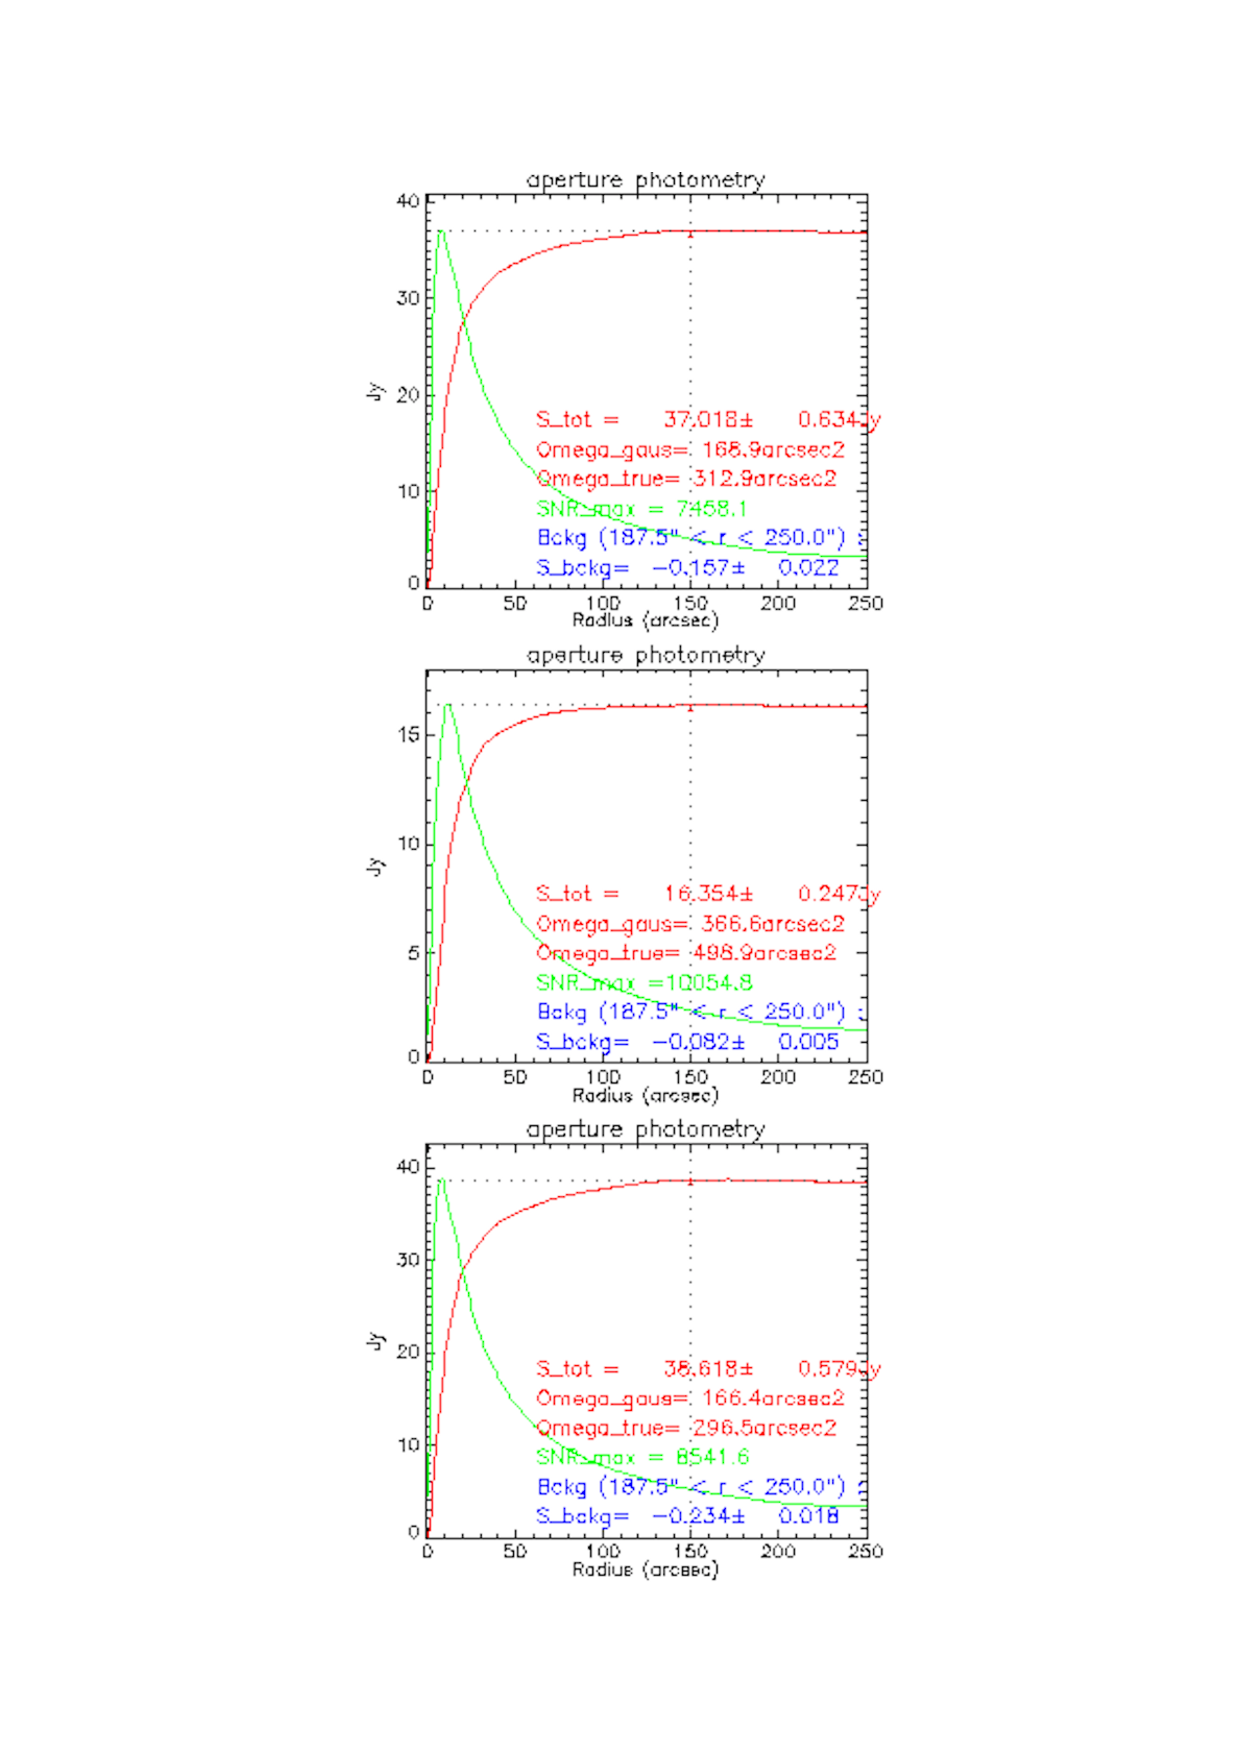
\includegraphics[clip, angle=0, scale=0.4]{Figures/Uranus_s308.pdf}
  \caption{Aperture photometry of Uranus observation 20170227s308  on array 1, 2 and 3 from left to right.
    The photometric curve in red saturates at about the radial distance of  $150''$. (Green curve is the SNR in individual annulus}
\label{fig:PhAp}
\end{center}
\end{figure}

%\subsection{Attempt to determine elevation-gain curve with secondary calibrator ???}


\subsection{Stability of the flux density scale with the primary calibrators Uranus and Neptune }

The primary calibrators Uranus and Neptune are the best sources to caracterize the stability of the intrument
%because their flux densities can be accurately predicted at any date from Morenos's models (see \S~\ref{se:cal_HA})
because they are significantly stronger than the other calibrators.
We have caracterized the stability of NIKA2  in estimating the ratios between their measured 
and predicted flux densities. The measured flux densities are from aperture photometry of the
18 observations  of Uranus and Neptune of runs 9 and 10. These observations are   beammaps  (20min) and integrated sequences of 4 consecutive otf's 
(16min) providing comparable integration times. The aperture radius was as large $150''$ to reach saturation level
as illustrated in Fig.~\ref{fig:PhAp}. 

The stability of the flux density scale during these two runs 
is shown  in  Fig.~\ref{fig:U_N_ratio}  where all the flux density ratios of Uranus and Neptune are
plotted sequentially.
We found that the resulting mean ratios $\mu$ are close to unity,  1.005, 1.007, 1.034, for array 1, 2, 3, respectively,
indicating that the planet flux densities used to set the Jansky scale 
early in the data processing by the pipeline have been properly recovered. This fact is not obvious from basic principle and need to be better
understood. Additionnally, the scatter (rms) around these mean ratios are indicative of
the stability and are better than 4.5\%, 5.0\%, 6.6\% for array 1, 2, 3,
respectively. This stability is comparable to the level achieved by other modern instruments,
e.g. SCUBA2 (Dempsey, 2013).

It is noticeable that the two runs used for this caracterization  are
separated by two months and that the instrument underwent a warm up in between. It is also noticeable that the
atmospheric conditions significantly change ; it changed from fair weather during run 9 in february 2017
($0.05 < \tau_{1mm} < 0.35$) to mediocre weather during run 10 in April 2017 ($0.3 < \tau_{1mm} < 0.65$). 
A detailed analysis shows that scatters around means 
are about twice smaller in the first run (fair) than during the second run (mediocre) ;
precisely, stabilities for the first run
are 3.6\%, 2.5\% and 2.9\% for arrays 1, 2, 3, respectively,
and, correspondingly, for the second run, are  5.3\%, 6.7\% and 8.6\%.
It is thought, at the moment, that limitations in stability must be  caused by residual atmospheric fluctuations
in the astronomical signal and small uncertainty in opacity corrections.

Also, we have plotted these flux density ratios versus elevation, opacity and attenuation in  Fig.~\ref{fig:ratio_vs_att}.
No clear correlation is apparent. The possible correlations of $\Omega_{true}$ at small opacity seen in Fig.~\ref{fig:Otrue}
are not apparent here. This is an indication that changes in $\Omega_{true}$, possibly 
caused by telescope surface deformations and atmospheric conditions, have been modelled
to some degree of accuracy and  the effect removed. We stress again that no gain-elevation curve was applied
in processing the data but that  $\Omega_{true}$ was determined for each observation and must modelled its slight variability
through the runs.

In addition to these fluctuations, the other limitation of the Jy scale is absolute calibration that depends on the
accuracy of the Moreno's model used to  predict the reference flux density of Uranus and Neptune (see \S~\ref{se:cal_HA})    
which is estimated to be 5\% in the millimeter wavelength range.
Hence, in combining quadratically both limitations (stability and absolute flux density),
the total uncertainty of calibration of NIKA2 is $10\%$ in mediocre atmospheric
condition and better than $6\%$ in fair condition as characterized with runs 9 and 10.

Correlations between flux density ratios of the three arrays are shown in Fig.~\ref{fig:U_N_corr}, separately
for runs 9 and  10. Highest correlations are found between arrays 1 and 3.

Finally, as already mentioned, we have all integrated sequences of 4 consecutive otf's of Uranus
acquired during run 9 to make their integration time (16 min) comparable to beammaps (20min). The intention was
to have similar  statistical error for all observations.  For the sake of completness, we have redone the stability study
in keeping separate all individual 4 minute long otf's.
The resulting flux density ratios are shown in Fig.~\ref{fig:U_otf_indiv}
and their means and rms are found to be totally consistent with our previous estimates.
Slight systematics may be more apparent. Additional observations of the planets in the
future will be useful to discuss this effect.


\begin{figure}
\begin{center}
  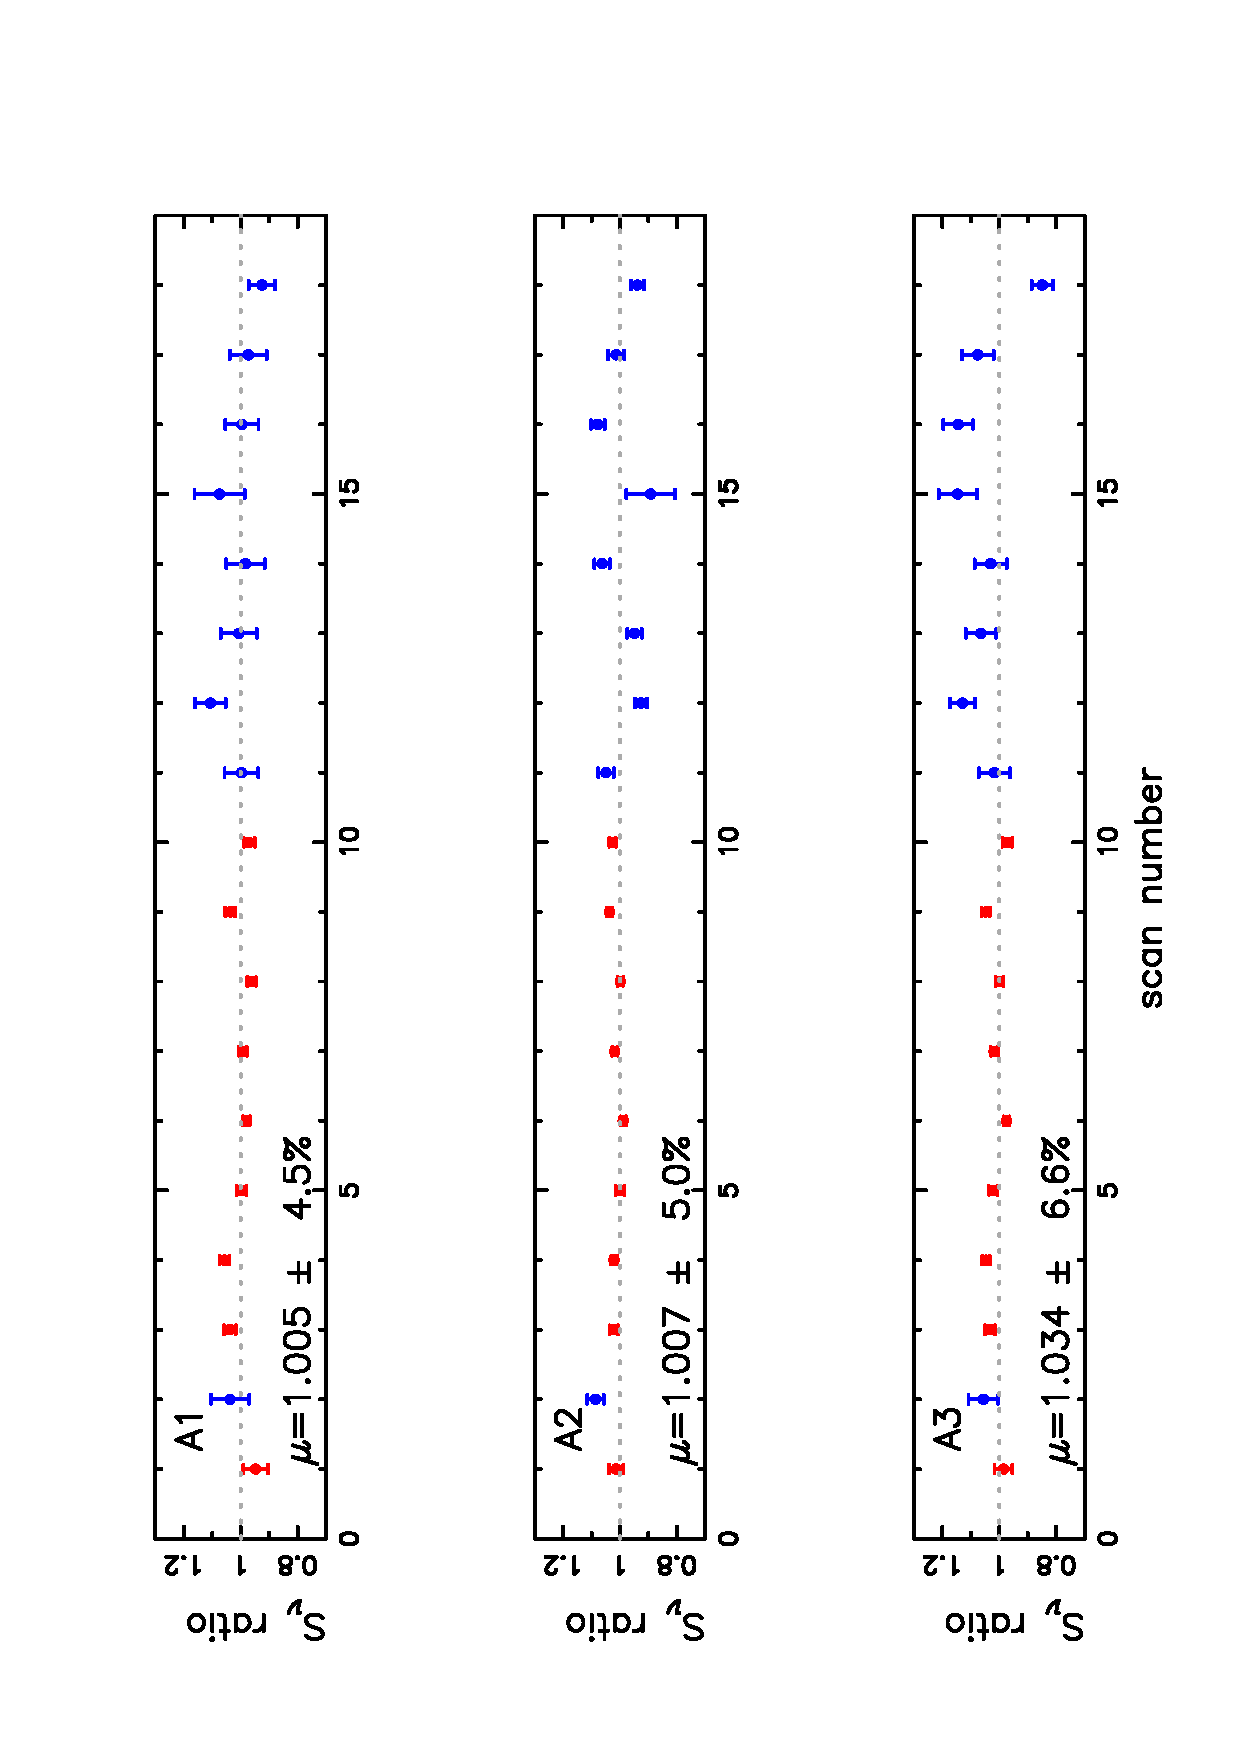
\includegraphics[clip, angle=-90, scale=0.6]{Figures/Ura_Nept_r9_10.pdf}
  \caption{Stability of the flux density scale with the primary calibrators Uranus (red) and Neptune (blue) :
    ratios between their measured and reference flux densities during run 9 and 10.
    Mean ratio $\mu$ and scatter are provided for each array.
    Observation numbers are time ordered : 1 to 10 are 23-28 february 2017 and 11 to 18 are 19-25 april 2017.
    Neptune was hardly visible at the telescope during run 9, and Uranus was not visible during run 10.
    Observations are beammaps (22 minutes) or sequence of 4 consecutive 4 minute long otfs (16 miunutes) that are
    comparable in integration times.}
\label{fig:U_N_ratio}
\end{center}
\end{figure}

\begin{figure}
\begin{center}
  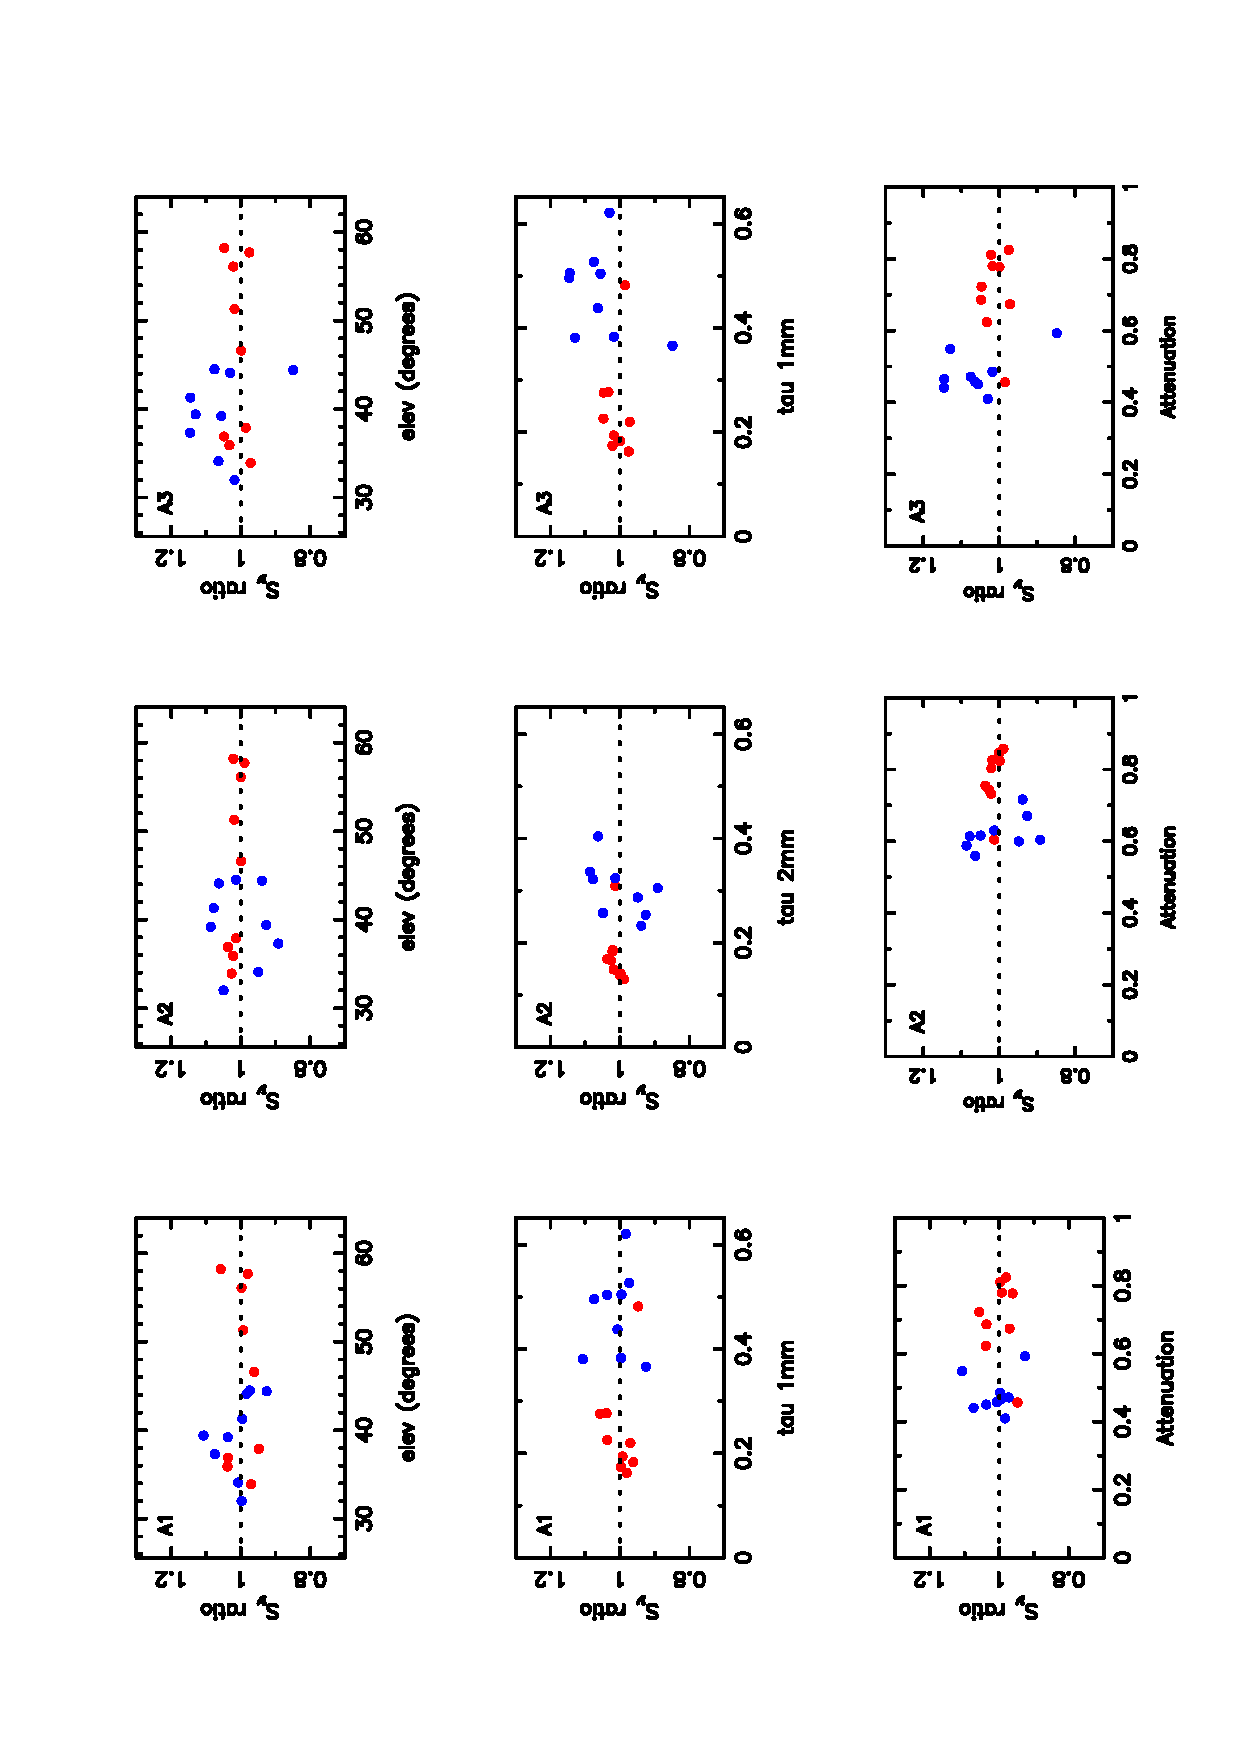
\includegraphics[clip, angle=-90, scale=0.6]{Figures/Ura_Nep_ratio_vs_elev_tau_attenuation_r9_r10.pdf}
  \caption{Flux density ratios versus elevation, opacity, and attenuation ($exp(-\tau/sin(elev)$) for Uranus and Neptune.
    No correlation is apparent with attenuation.}
\label{fig:ratio_vs_att}
\end{center}
\end{figure}


\begin{figure}
\begin{center}                                                                                                             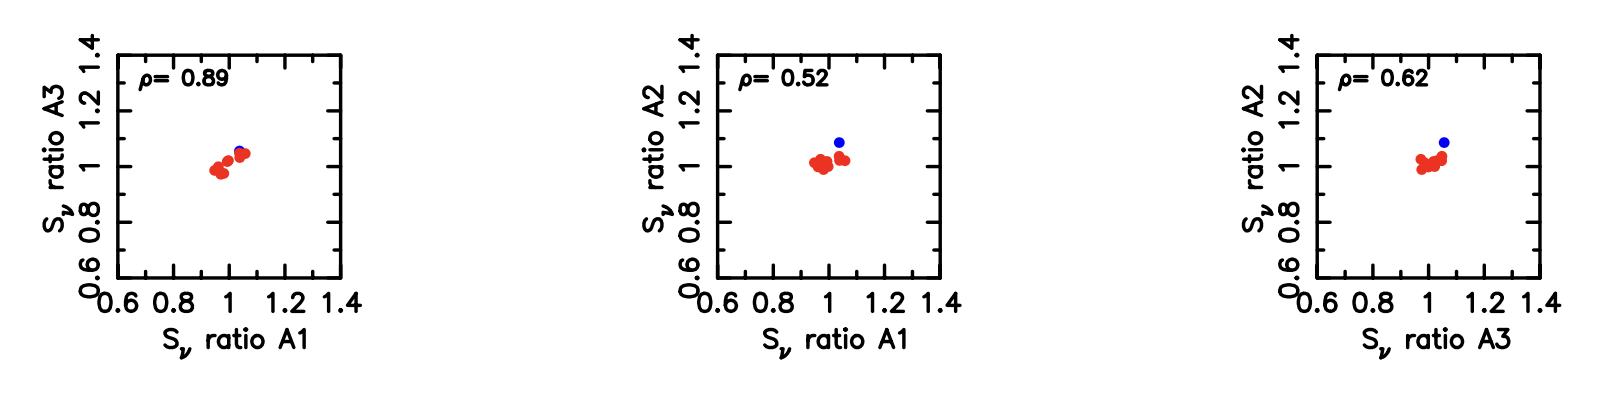
\includegraphics[clip, angle=0, scale=0.55]{Figures/Corr_r9.png}
  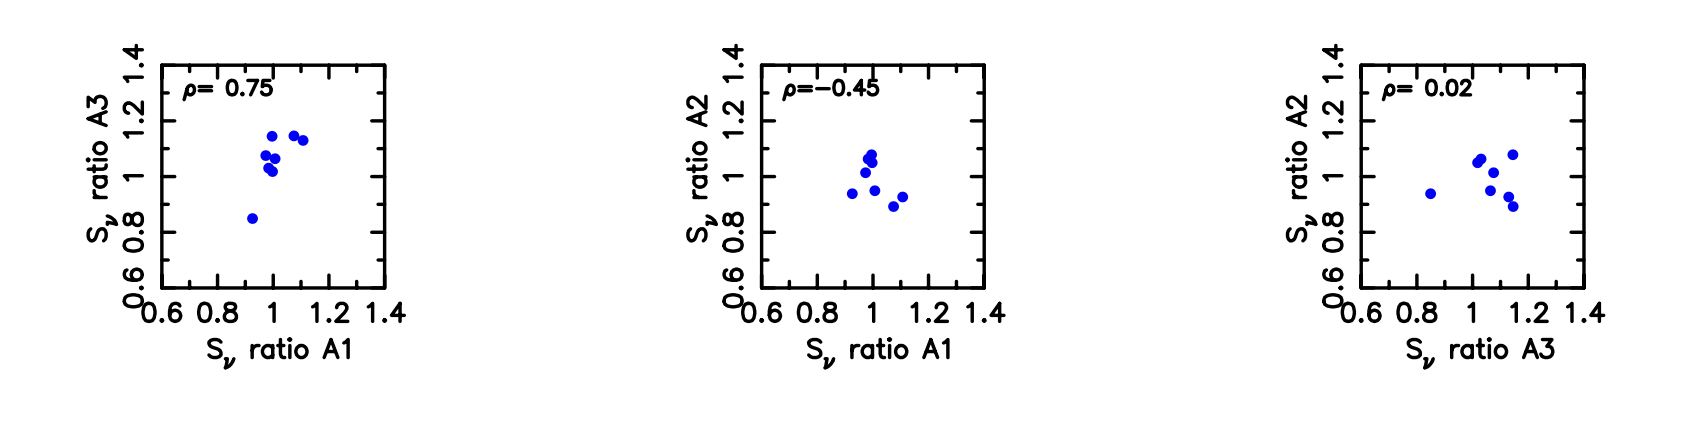
\includegraphics[clip, angle=0, scale=0.55]{Figures/Corr_r10.png}  
  \caption{Correlation plots for the flux density ratios between  the three arrays
    shown separately for run 9 (fair atmospheric condition) and run 10 (mediocre condition).
    Correlation coefficients $\rho$ are given.}
\label{fig:U_N_corr}
\end{center}                                                                                                             \end{figure}


\begin{figure}
\begin{center}
  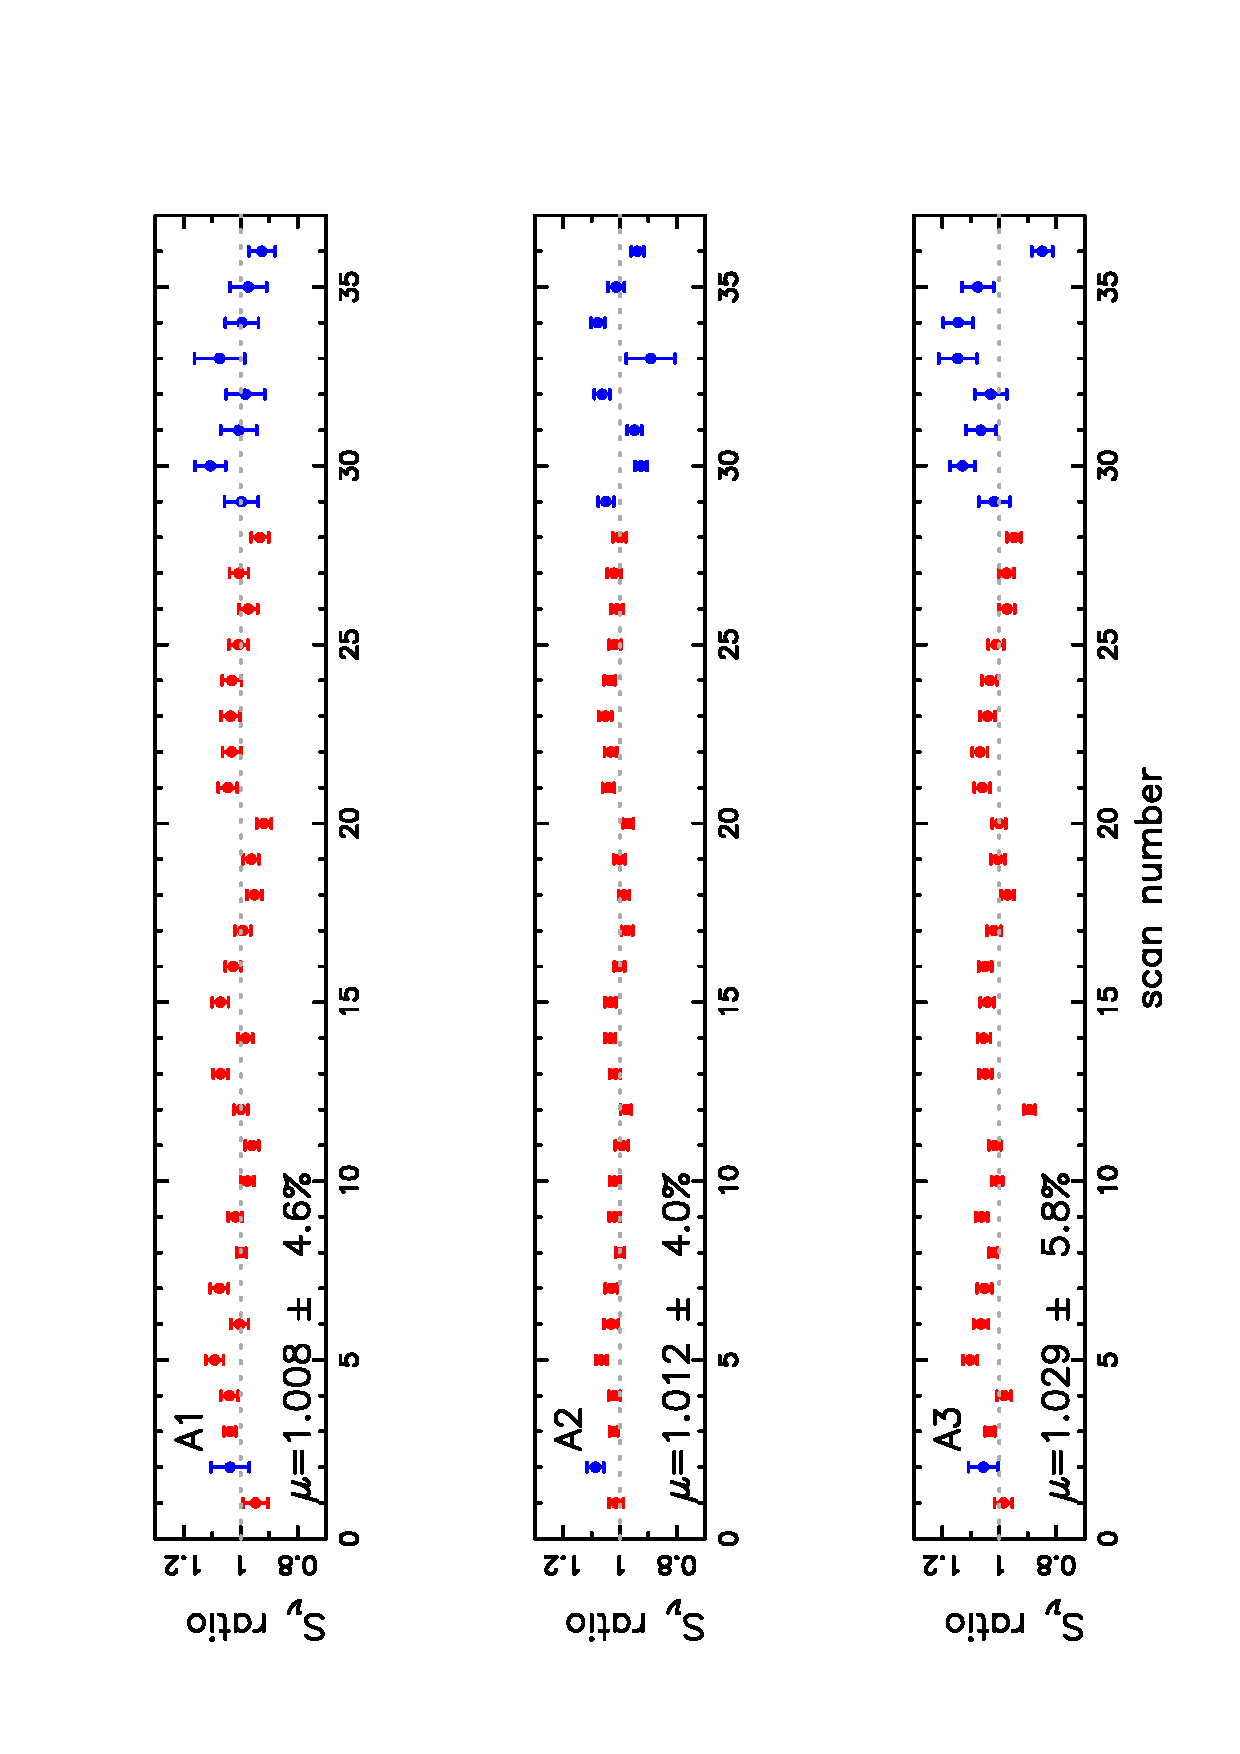
\includegraphics[clip, angle=-90, scale=0.6]{Figures/Flux_ratio_index_A1_A2_A3.pdf}
  \caption{Stability of the flux density scale with the primary calibrators Uranus (red) and Neptune (blue).
    Here, single 4 minute long otf's of Uranus acquired during run 9 are kept separate
    and displayed, while, in Fig.\ref{fig:U_N_ratio} above, 4 consecutive otf's were integrated together (16 min).
    Means and rms of flux density ratios are not significantly different though.}
\label{fig:U_otf_indiv}
\end{center}
\end{figure}

\subsection{Flux densities of secondary calibrators MWC349, NGC7027 and CRL2688 calibrated with Uranus and Neptune}

The sources  MWC349, NGC7027 and CRL2688 are standard secondary calibrators
and were observed during runs 9 and 10. Their flux densities at the NIKA2 reference frequencies 150 and 260 GHz
have been predicted  in using data from the literature
in Table~\ref{tab:flux_ref_sec} (see \S~\ref{se:fluxSec}).  Also, we stress that MWC349 is a flux density calibrator at PdB and
the current measurements of its monitoring program have been used for its prediction \cite{krips}.
In runs 9 ab 10, there are 34 and 37 observations of these secondary calibrators, respectively, after nine observations were discarded because
aperture photometry failed.

As for the planets, the observations were processed with the pipeline set up with the parameters
of Table~\ref{tab:Pipe}. For this processing,
the two kidpars used ({\it kidpar-best3files-FXDC0C1-GaussPhot, kidpar-n2r10-calib})  include the conversion factors
from Hz to Jy that were calibrated with Uranus and Neptune flux densities predicted at the central frequencies
of the bandpasses, 255, 152 and 258~GHz for arrays 1, 2,
and 3,  respectively. It is only after this processing that it was decided to abandon central frequencies
and to choose the reference frequencies 260 and 150~GHz for the NIKA2 1 and 2mm  bands (see \S~\ref{se:cal_HA}).

The flux densities of these secondary calibrators measured with  aperture photometry are in Table~\ref{tab:flux_sec_Ap},
and those measured with  the pipeline are in Table~\ref{tab:flux_sec_NK}. For aperture photometry, the solid angle $\Omega_{true}$
was determined from the NIKA2 map of each observation.
In these tables, the flux densities have been corrected for the change from
the central frequency $\nu_c$ (255,152, 258GHz) to the NIKA2 reference frequency $\nu_{ref}$ (150, 260GHz), {\it i.e.}
$\Delta S_{\nu}  = \alpha S_{\nu} (\nu_{ref}-\nu_c)/\nu_c $) with the spectral index $\alpha$ defined
as $S_{\nu} \propto \nu^{\alpha}$ (see Table \ref{tab:flux_ref_sec}). These changes are less than 5\%.
Color-corrections have also been applied
with indices $\alpha=+0.6$, $-0.34$ and $+2.44$ for MWC349, NGC7027 and CRL2688, respectively, while Uranus and
Neptune have $\alpha=+1.6$. These corrections are smaller than 2.5\% (see Table in
\S~\ref{se:cal_HA}, CAUTION : this table is pending in  HA section).  Again, both of these corrections are included
in Tables~\ref{tab:flux_sec_Ap} and \ref{tab:flux_sec_NK} where the flux densities and uncertainties are the mean and rms
of all observations of each source during each run. Note finally that each observations is the integration of 4 consecutive otf's (total 16 minutes). 


\begin{table}[h]
\centering
\caption[]{Flux densities from {\bf aperture photometry} and relative differences in percent with respect to reference values.}
\begin{tabular}{|c|c|c|c|c|c|}
\hline
\multicolumn{3}{|c}{}  & \multicolumn{3}{|c|}{Flux densities (Jy)}   \\
\hline
         & run  & \#obs &  A1                    &  A2                   &    A3                    \\
         &      &      &  $S_{260 {\rm GHz}}$     &  $S_{150 {\rm GHz}}$  & $S_{260 {\rm GHz}}$    \\
\hline
MWC349   &  9   & 10  &  $2.23\pm0.32$  ($+8.2\%$)  &  $1.49\pm0.11$ ($+0.6\%$) &  $2.15\pm0.35$ ($+4.6\%$)      \\
  $''$   & 10   & 14  &  $1.96\pm0.17$  ($-4.8\%$)  &  $1.48\pm0.08$ ($+0.2\%$) &  $2.10\pm0.19$ ($+1.8\%$)                  \\
         &      &     &                             &                           &                            \\
NGC7027  &  9   & 13  &  $3.22\pm0.39$  ($-6.9\%$)  &  $4.19\pm0.18$ ($-1.6\%$) & $3.05\pm0.54$  ($-11.9\%$)      \\
  $''$   & 10   & 15  &  $3.01\pm0.36$  ($-13.0\%$) &  $4.04\pm0.30$ ($-5.2\%$) & $3.31\pm0.19$  ($-4.2\%$)                   \\
         &      &     &                             &                           &                                 \\
CRL2688  &  9   & 11  &  $2.91\pm0.48$  ($-0.1\%$)  &  $0.59\pm0.05$ ($-22.9\%$)  &  $2.68\pm0.51$ ($-7.9\%$)     \\
  $''$   & 10   &  8  &  $2.36\pm0.14$  ($-19.0\%$) &  $0.52\pm0.04$ ($-32.1\%$)  &  $2.49\pm0.18$ ($-14.5\%$)                   \\
\hline
\end{tabular}
\label{tab:flux_sec_Ap}
\end{table}
%open(1,file='sequence_Ur_Nep_r_8_9_10.dat' (contient aussi cal sec du r 9 seulement)  ;  flux=flux
% open(1,file='run10_cal_sec.dat')    ! kidpar_n2r10_calib (mask=50") with F2D, bramax (seul fichier avec cela)    
% cahier II p. 46, 47 : corrections (255, 258GHz) --> 260GHz  (152GHz) --> 150GHz  and color-correction with Table p.37


\begin{table}[h]
\centering
\caption[]{Flux densities from {\bf pipeline} and relative differences in percent with respect to reference values.}
\begin{tabular}{|c|c|c|c|c|c|}
\hline
\multicolumn{3}{|c}{}  & \multicolumn{3}{|c|}{Flux  densities (Jy)}   \\
\hline
         & run  & \#obs &  A1                        &  A2                        &           A3                  \\
         &      &       &  $S_{260 {\rm GHz}}$       &  $S_{150 {\rm GHz}}$       & $S_{260 {\rm GHz}}$         \\
\hline  
MWC349   &  9   & 10    &  $1.98\pm0.16$ ($-4.1\%$)  &  $1.46\pm0.05$ ($-1.3\%$)  &  $2.02\pm0.17$ ($-2.0\%$)     \\
  $''$   & 10   & 14    &  $1.71\pm0.16$ ($-16.8\%$) & $1.44\pm0.05$ ($-2.5\%$)   &  $1.84\pm0.20$ ($-10.7\%$)      \\
         &      &       &                            &                            &                              \\
NGC7027  &  9   & 13    &  $3.53\pm0.33$ ($+2.1\%$)  &  $4.28\pm0.18$ ($+0.4\%$)  & $3.62\pm0.36$ ($+4.7\%$)      \\
  $''$   & 10   & 15    &  $3.27\pm0.19$ ($-5.5\%$)  & $4.28\pm0.14$ ($+0.6\%$)   &  $3.53\pm0.19$ ($+2.1\%$)        \\
         &      &       &                            &                            &                                \\
CRL2688  &  9   & 11    &  $2.53\pm0.23$ ($-17.0\%$) &  $0.55\pm0.02$ ($-27.5\%$) &  $2.49\pm0.24$ ($-14.2\%$)    \\
  $''$   & 10   &  8    &  $2.22\pm0.12$ ($-23.6\%$) &  $0.54\pm0.02$ ($-29.3\%$) &  $2.32\pm0.13$ ($-20.4\%$)     \\
\hline
\end{tabular}
\label{tab:flux_sec_NK}
\end{table}
%open(1,file='sequence_Ur_Nep_r_8_9_10.dat' (contient aussi cal sec du run 9 seulement) ;   flux=S_NK
% open(1,file='run10_cal_sec.dat')    ! kidpar_n2r10_calib (mask=50") with F2D, bramax (seul fichier avec cela) 

From these two Tables, we conclude that  the 2 mm flux densities of MWC349 and NGC7027 measured with array 2 are consistent with predictions,
and consistent between runs (9 and 10) and methods (aperture photometry, pipeline Gaussian fit) at the few percent level
($(S_{meas}-S_{ref})/S_{ref} \times 100)$. But this is not the case for CRL2688.  Its NIKA2 2mm
flux density is $\sim$25\% lower than prediction, consistently between runs and methods. Hence, this may be due to an over estimation
in the prediction of the 2 mm flux density that was extrapolated from the SCUBA2 850 $\mu$m and 450 $\mu$m measurements
and because of the large lever arm in frequency. We note this
over estimation seems to be also true at 1mm for this source in the two Tables.
Future observations of CRL2688 will check wether or not its new NIKA2 flux densities are valid to populate usefully its SED
for science purpose. 

For the 1 mm flux densities of MWC349 and NGC7027 from these two tables, we conclude that their  measurements with arrays 1 and 3 are
at the 10\% level   ($(S_{meas}-S_{ref})/S_{ref} \times 100)$  and are consistent with statistical uncertainties estimated from
the rms of their fluctuations
during the two runs and shown in Fig.~\ref{fig:ratio_cal_sec}. For example, NGC7027, A1, run 10, aperture photometry in Table~\ref{tab:flux_sec_Ap}
yields  :

$$rms(S_{obs})/<S_{obs}>=0.36Jy/3.01Jy \times 100=11.9\%$$

\noindent which is statistically consistent with :

$$|(S_{meas}-S_{ref})/S_{ref}| \times 100=15.0\%~,$$

\noindent where $S_{meas} = <S_{obs}>$.

Finally, we have plotted the flux density ratios versus elevation, opacity and attenuation  for three
secondary calibrators in  Fig.~\ref{fig:corr_cal_sec}. No clear correlation is apparent.

\begin{figure}
\begin{center}
  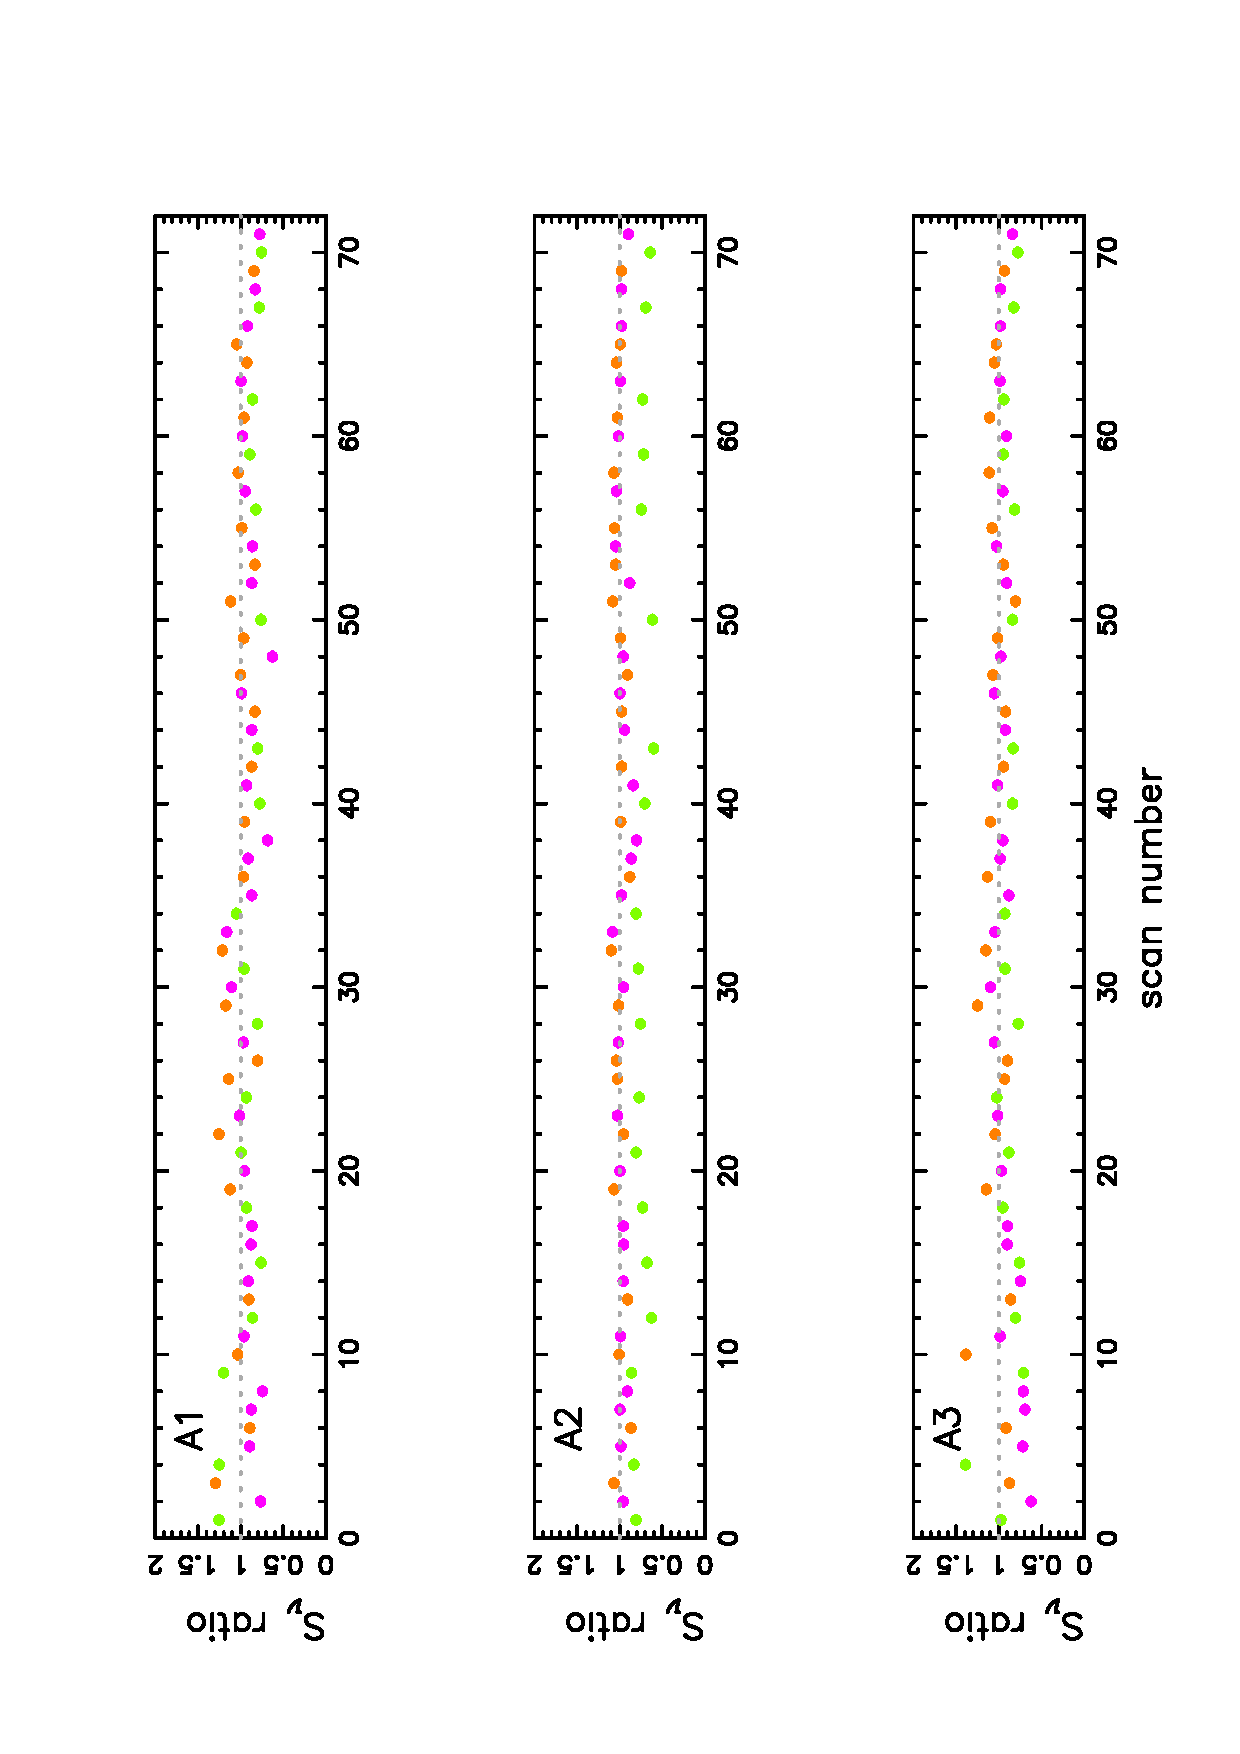
\includegraphics[clip, angle=-90, scale=0.6]{Figures/Ratio_vs_index_sec_r9_r10.pdf}
  \caption{Ratios between measured and reference flux densities of  the secondary calibrators  MWC349 (brown), NGC7027 (purple)  and CRL2688 (green)
  during runs 9 and 10. As discussed in text, CRL2688 (green) is about 25\% lower than the flux density predicted from SCUBA2 at other higher frequencies.
  If confirmed in further runs, the NIKA2 2mm flux density will usefully populate the SED of this source.  
    Scan numbers are time ordered (index 1 to 34 : run 9 (fair weather) and index 35 to 71 : run 10 (mediocre weather).
    Degradation with worst atmospheric conditions is not as apparent as for Uranus and Neptune.
    Each observation is a sequence of 4 consecutive 4 minute long otfs (total integration is 16 minutes).}
\label{fig:ratio_cal_sec}
\end{center}
\end{figure}


\begin{figure}
\begin{center}
  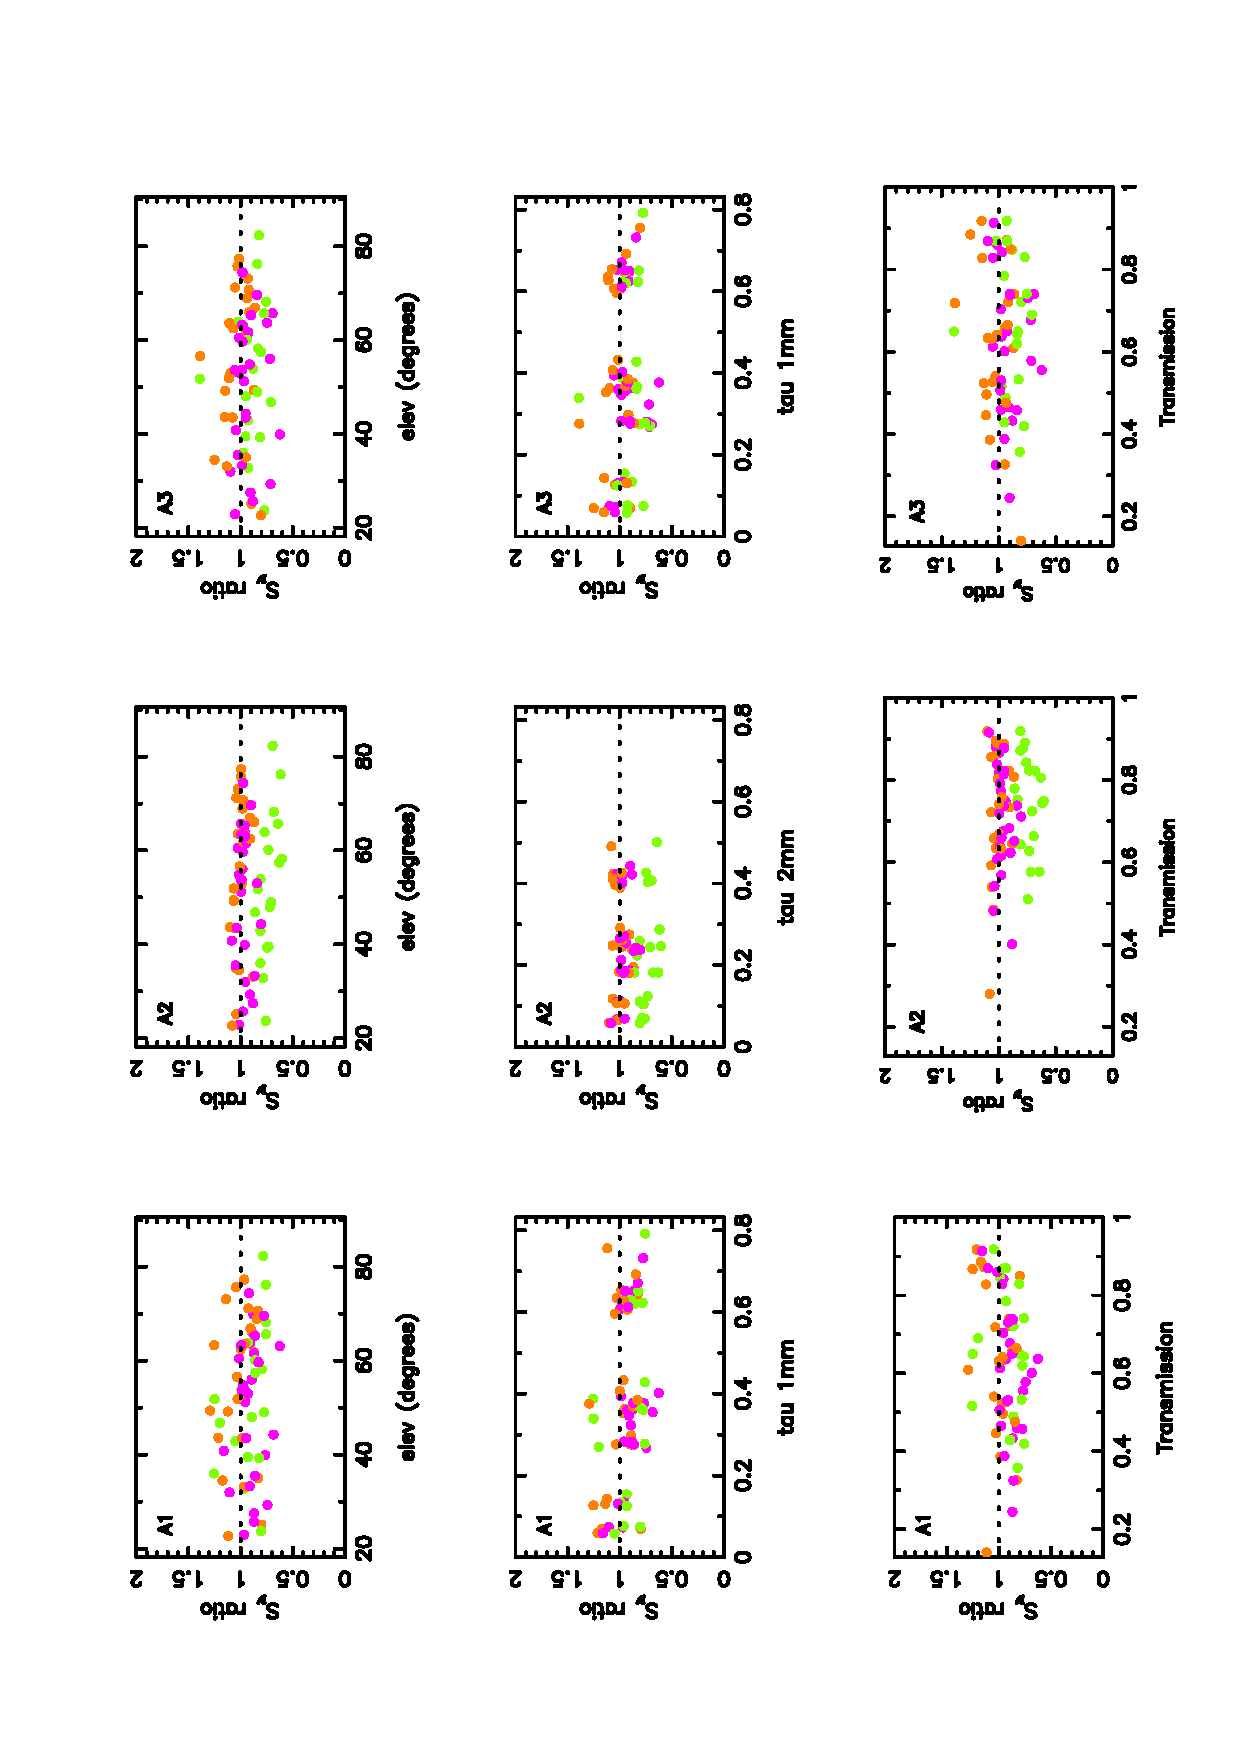
\includegraphics[clip, angle=-90, scale=0.6]{Figures/Ratio_vs_elev_op_sec_r9_r10.pdf}
  \caption{Flux density ratios versus elevation, opacity, and attenuation ($exp(-\tau/sin(elev)$) for the three secondary
    calibrators  MWC349 (brown), NGC7027 (purple)  and CRL2688 (green) during run 9 ($0.05  < \tau_{1mm} < 0.35$)
    and run 10 ($0.35  < \tau_{1mm} < 0.80$). No clear  correlation is apparent. See comment on CRL2688 (green) in legend of Fig.\ref{fig:ratio_cal_sec}
    and text.}
\label{fig:corr_cal_sec}
\end{center}
\end{figure}

















